\documentclass{sig-alternate}

\begin{document}

\title{Deployment Experiment of an Elastic Cloud Application}
\subtitle{Technical University of Vienna,\\Advanced Internet Computing,\\
(Jan 2013)}


\numberofauthors{4}
\author{
\alignauthor
Soodeh Farokhi\titlenote{In alphabetical order}\\ %or put the group leader first, if you wish
       1228800
\alignauthor
Gajo Gajic\\
       0828150
\and
\alignauthor
Martin Kalany\\
       0825673
\alignauthor
Jia Wei\\
       0035204
}
       
\date{\today}

\maketitle
\begin{abstract}
\end{abstract}

Scalability is said to be one of the major advantages brought by the cloud paradigm and, more specifically, the one that makes it different to an “advanced outsourcing” solution~\cite{vaquero2011dynamically}.

\section{Introduction}

goal: providing scalable software platforms in clouds


\subsection{CloudScale Features}
1. CloudScale, on the other hand, allows application developers to retain full control over their application. CloudScale applications are not bound to any specific cloud provider, are easy to migrate, work well in the context of private or hybrid clouds, and support a wider variety of applications, while still providing an abstraction comparable to commercial PaaS solutions \cite{Leitner2013}..\\

2. The main disadvantage of all of those systems is that they imply a significant loss of control for the developer and also they typically require the usage of a given public cloud (typically provided by the same vendor), imply the usage of propri- etary APIs, and restrict the types of applications that are supported \cite{Leitner2013}.

3. CloudScale middleware for transparently scaling applications using an IaaS cloud.

4. The CloudScale approach provides a middle ground between common IaaS offerings, which provide great control over the application, but do so at the costs of high deployment effort, and PaaS offerings, which are easy to use, but provide little control. ~\cite{leitner2012cloudscale}



\section{State of the art}


There are essentially two schools of thought of how one should build any distributed system. On the one hand,many approaches aim at hiding the complexity of distribution be- hind convenient abstractions, such as remote procedure call systems. On the other hand, some claim that such abstractions always have to be leaky, and, hence, should be avoided altogether. we follow the former school of thought. Essentially, CloudScale provides an abstraction that makes elastic applications running on top of an IaaS cloud seem like regular, non-distributed Java applications.

The possible mechanisms for scalability of applications in Clouds has been depicted in Fig.\ref{fig:scalabilitymechanisms}, and CloudScale approach falls into "container replication" category in the platform layer (the container being CloudScale in this case) as well as Aneka and AppScale.

\begin{figure*}
\centering
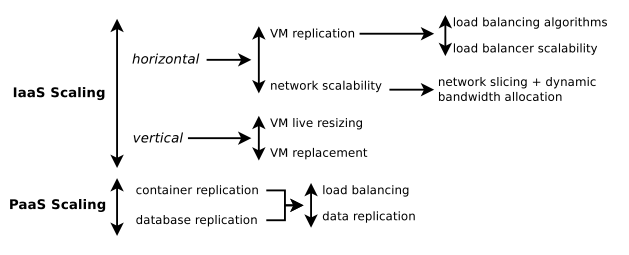
\epsfig{file=figures/ScalabilityMechanisms.png}
\caption{Available Mechanisms for Holistic Application Scalability ~\cite{vaquero2011dynamically}}
\label{fig:scalabilitymechanisms}
\end{figure*}

\subsection{Container-level Scalability}
This category is like CloudScale approach (description of this kind of approach is described in \cite{vaquero2011dynamically}.

Aneka \cite{vecchiola2009aneka}: For high loads, and to avoid overprovisioning of resources, it would be useful to be able to federate clouds so components can be run in external/public clouds if needed. Aneka is able to deploy containers and run users applications in several IaaS providers \cite{vaquero2011dynamically}. 

AppScale \cite{chohan2009appscale}: Platforms will require container replicas to be deployed or released dynamically to handle load variations. AppScale can scale the VMs used to host containers depending on actual application demand, automatically configuring the load balancers \cite{vaquero2011dynamically}. 


We can consider two main categories for the WR: 
\subsection{Related Research (scientific approaches)}

(1) paper \cite{miranda2012enough} (MDA): Enough about standardization, let's build cloud applications

(2) paper \cite{keller2013topology}:(cite CloudScale) A topology-aware adaptive deployment framework for elastic applications 

(2-1) \textbf{Ubuntu Juju }\footnote{https://juju.ubuntu.com/}: Basic services are described as predefined charms

(2-2) \textbf{RIM. Carina Environment Manager} \footnote{https://github.com/blackberry/OpenNebula-Carina}: It automate and speed up the deployment of services onto the OpenNebula private clouds

(2-3) CA 3Teras\textbf{•} \footnote{http://www.ca.com/us/cloud-platform.aspx}: 3Teras AppLogic automates complex application deployment.

(2-4)\textbf{Aeolus} /cite{di2012towards}: Aeolus’s component model specifies compositions of services to automate deployments, planning of day-to-day activities such as software upgrade planning, service deployment, elastic scaling
 
(3)Is your cloud elastic enough?: performance modelling the elasticity of infrastructure as a service (IaaS) cloud applications \cite{brebner2012your}

(4)Component-based scalability for cloud applications \cite {kachele2013component}

(5)Look up!: your future is in the cloud \cite{larus2013look}

(6)Orleans: cloud computing for everyone \cite{bykov2011orleans}

(7)Lightweight Resource Scaling for Cloud Applications \cite{han2012lightweight}
 
\textbf{Aneka} is a .NET-based platform with a focus on enabling hybrid cloud applications. Unlike CloudScale, Aneka is more akin to traditional Grid computing middleware, providing a relatively low-level abstraction based on the message passing interface (MPI). In general, Aneka seems suitable for building scientific computing applications, but less so for enterprise applications ~\cite{Leitner2013}

\textbf{AppScale}, on the other hand, specifi- cally (and exclusively) targets Online Transaction Processing (OLTP) style enterprise applications ~\cite{Leitner2013}.
 
another platform with a focus on data processing has been proposed by the BOOM research project [4]. BOOM builds on a custom, declarative programming model and is clearly geared towards data analytics ~\cite{Leitner2013}..

The main contribution of CloudScale over all of these models is that Cloud- Scale has amore general claim, and is able to handle a wide variety of elastic application types, including data-intense, processing-intense and OLTP style web applications ~\cite{Leitner2013}.. 

The European commission funded project \textbf{Contrail} [2] is currently building another PaaS for hosting relatively flexi- ble elastic applications, called ConPaaS [28] (Contrail PaaS). ConPaaS supports web and high-performance applications built in Java or PHP, and can be used in combination with Amazon EC2 or an OpenNebula private cloud. However, ConPaaS seems to operate on a lower level of abstraction than CloudScale. This PaaS environment consists of elas- tically hostedWeb services, such as web or database servers, and mostly integrates existing stand-alone components \cite{Leitner2013}.


\subsection{Related tools and commercial approaches}

A service particularly related to our work is \textbf{CloudBees RUN@Cloud} \footnote{http://www.cloudbees.com/}, which provides continuous integration and an elastic platform for hosting Enterprise Java Beans (EJB) applications \cite{Leitner2013}.

Other PaaS of- ferings that support the Java programming language include the well-known GAE, Amazon’s Elastic Beanstalk services, or Microsoft’s Azure \cite{Leitner2013}. 

Outside of the Java world,\textbf{ Heroku} is gaining traction as a provider of PaaS for dynamic scripting languages, such as Ruby or Python\footnote{https://www.heroku.com/} \cite{Leitner2013}.

AppScale can be also considered as a commercial product and it allows users to build their own GAE compliant PaaS on top of any private or public IaaS service. We consider this system a significant step forward in comparison to other vendors \cite{Leitner2013}.

Many core features and terms of CloudScale, as introduced in Section 3.1, are akin to well-known Java remote procedure call technology, e.g., Java RMI or EJB. How- ever, note that the main contribution of CloudScale is not in enabling remoting (as RMI and EJB do), but rather in enabling elasticity. Hence, the actual conceptual overlap between CloudScale and these frameworks is not particularly large.
In this paper, we more focus on the first category by investigating the scientific state of the art in elastic cloud applications, while just introduce some existing tools and technologies for the second category \cite{Leitner2013}.



\subsection{Other aspects}
1. efficiently deploying applications in the cloud

2. distributed deployment and hosting of (Java) applications: most replicating and clustering of \textbf{Enterprise Java Beans} (EJB) implementations lack the dynamism of CloudScale, and do not provide resource management strategies or transparent code distribution \cite{leitner2012cloudscale}.

3. Specialized programming models: \textbf{Aneka} is a platform for deployment of .NET-based applications, employing a specialized programming model. The BOOM initiative at UC Berkeley aims at simplifying declarative programming for the cloud. Whereas BOOM is mostly suited for data analytics, Cloud- Scale is targeted at general-purpose programming and deployment of arbitrary Java applications \cite{leitner2012cloudscale}. 

4. PaaS and SaaS: From a technical viewpoint, these providers do little more than allowing scalable remote access to existing software developing platforms, enriched with rich user interface and Web 2.0 experience; The main difference between CloudScale and those commercial SaaS and PaaS solutions is that, when using CloudScale, developers retain full control over their application. That is, even though CloudScale hides some scalability-related issues from developers, they are still free to customize the way CloudScale works to their own needs, either by implementing customscaling policies, adapting the CloudScale framework itself, or managing some COs in the application manually \cite{leitner2012cloudscale}. 

5. Java-based remoting: e.g.,\textbf{ Java RMI, Enterprise Java Beans} (EJB) or CORBA. These frameworks, while technically similar, provide only limited support for automated scaling. How- ever, the ideas behind the CloudScale middleware could be implemented on top of these technologies, enhancing, e.g., the CORBA remoting model with automated load balancing in the cloud.




\section{Conclusion}

%bibliography
\bibliographystyle{abbrv}
\bibliography{sigproc} 
\end{document}
